
\section{Methodlogy}

\begin{figure*}[!ht]
    \centering
    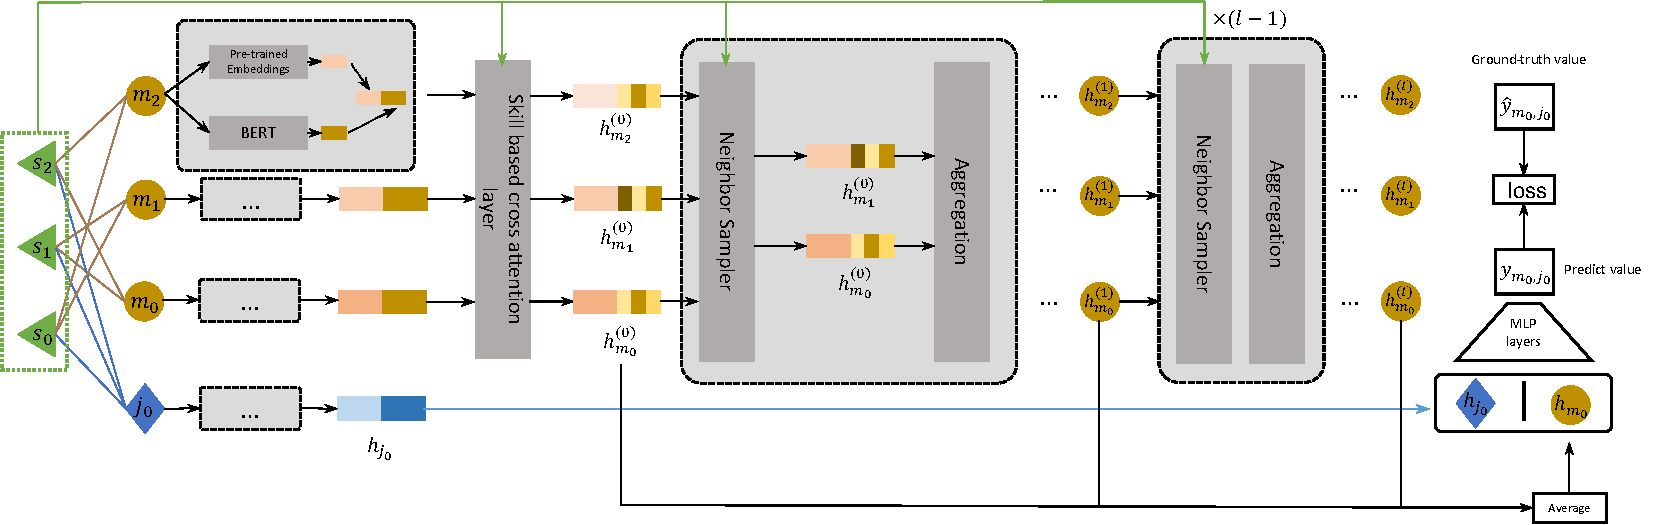
\includegraphics[width=0.75\textwidth]{fig/CSAGNN.pdf}
    \caption{Architecture of CSAGNN. When determining the match between job $j_0$ and member $m_0$, the information from $m_0$'s professional connections, $m_1$ and $m_2$, is simultaneously acquired. The initial representations of both the member and job are formed by concatenating the WHIN pre-training embedding with the representation obtained after processing the text information through BERT. All member text information is re-weighted through an attention mechanism based on the skills $s_i$ required by $j_0$. A neighbor sampler module, operating based on the similarity between different members and the required skills, can filter out professional connections that are not relevant to the job.}
    \label{fig:CSAGNN_framework}
\end{figure*}


Here we introduce our two-stage approach to improve the performance of the Person-Job Fit task by incorporating professional networks. The task and notation are formally defined in Section \ref{Formal Task Description and Notations}. In the first stage, we pre-train on the Workplace Heterogeneous Information Network (WHIN), which is detailed in Section \ref{The Construction of Workplace Heterogeneous Information Network}. We introduce the pre-training approach on WHIN in Section \ref{Pre-training on Workplace Heterogeneous Information Network}. To overcome the noise in professional networks, we propose the contextual social attention graph neural network (CSAGNN) in the second stage, as described in Section \ref{Contextual Social Attention Graph Neural Network}.

\subsection{Formal Task Description and Notations}
\label{Formal Task Description and Notations}
Person-Job Fit aims to match a set of job seekers with a set of job opportunities. Assume that there is a set of members $\mathcal{M}=\set*{m_1, m_2,\dots , m_n}$ who may be seeking job opportunities and a set of jobs $\mathcal{J}=\set*{j_1, j_2, \dots, j_m}$. Formally, given a candidate pair $(m_j, j_k)$, the model is required to learn a function $\mathcal{F}$ to predict the probability of whether the member applied for the job.
\[
    \mathcal{F}(m_i, j_k) =  \begin{cases}
        1 & m_i \text{ applied for } j_k \\
        0 & m_i \text{ didn't apply for } j_k
    \end{cases} \\
\]
The set of candidate pairs can be defined as

$$T=\set*{(m_i, j_k)|m_i\in \mathcal{M}, j_k\in \mathcal{J}}$$.

In addition to the sets of members ($\mathcal{M}$) and jobs ($\mathcal{J}$), there exist three other sets of entities that are strongly related to members and jobs: skills ($\mathcal{S}$), companies ($\mathcal{C}$), and schools ($\mathcal{H}$). These entities are referred as auxiliary information and can be leveraged to improve the model's accuracy. Given an entity $e$ and a relation $r$, an interaction map $\mathcal{A}_{e}^{r}$ is used to specify the destination entities related to $e$ through $r$. For example, $\mathcal{A}_{m_i}^{apply}$ represents the set of jobs applied by $m_i$. If $m_i$ has not applied for any jobs, $\mathcal{A}_{m_i}^{apply}=\emptyset$.

\subsection{The Construction of Workplace Heterogeneous Information Network}
\label{The Construction of Workplace Heterogeneous Information Network}

The Person-Job Fit scenario contains a wide range of heterogeneous knowledge, including various entities such as skills, companies, and schools, as well as relationships such as professional connections and skill requirements. We define a Workplace Heterogeneous Information Network (WHIN) to model this knowledge. As shown in Figure \ref{fig:metagraph}, WHIN is a heterogeneous information network consisting of five types of entities, namely Member, Job, Skill, Company, and School. It also contains nine types of relations, which are introduced to capture the different types of connections between the entities.
 
The Workplace Heterogeneous Information Network primarily consists of natural relations among diverse entities. Besides, two additional metapaths have been artificially constructed. The first metapath, co-apply ($\mathcal{M}$-$\mathcal{J}$-$\mathcal{M}$), connects members who have applied for the same job. The second metapath, co-applied ($\mathcal{J}$-$\mathcal{M}$-$\mathcal{J}$), connects multiple jobs that have been applied for by the same member. These metapaths were constructed based on prior knowledge and have proven to be useful in enhancing the performance of the WHIN pre-training process \cite{fu2020magnn}.

\subsection{Pre-training on Workplace Heterogeneous Information Network}
\label{Pre-training on Workplace Heterogeneous Information Network}

\subsubsection{link-level pre-training task}
\label{link-level pre-training task}
We utilize a heterogeneous graph neural network with a link-level pre-training task to acquire node representations with rich structural knowledge. To improve the scalability of the pre-training process, we create mini-batches by sampling subgraphs from the entire Workplace Heterogeneous Information Network (WHIN), as illustrated in Figure \ref{fig:WHIN_pretrain} (a) and (b).

Specifically, a batch of candidate pairs is selected as the source nodes. From these source nodes, their k-hop neighbors are sampled to construct a subgraph based on each direct relation or metapath. These identified relations and metapaths serve as positive samples. In addition, to introduce negative samples, we randomly select pairs of entities that do not exhibit the expected relationships. The link-level pre-training task revolves around determining the existence of the given samples. We employ an encoder-decoder structure, as illustrated in Figure \ref{fig:WHIN_pretrain} (c). The encoder learns node representations within each subgraph, while the decoder predicts link existence.

\subsubsection{pre-training model structure}
\label{pre-training model structure}

During the pre-training phase, we select a fixed number of tokens from the textual content of each entity type. These selected tokens are then processed through the BERT model \cite{devlin2018bert}. The resulting BERT outputs are averaged to create initial representations for each entity.

In a formal context, when working with a textual representation associated with an entity denoted as $e_i\in \mathcal{E}$, we construct a corresponding initial embedding referred to as $z_i^{(0)}$ by utilizing BERT. Specifically, We leverage member profiles, job descriptions, skill names, and other textual descriptions to initialize entity representations, thereby enhancing the initial embeddings for each entity type.

After obtaining an initialized representation with semantic information, we utilize an encoder, RGCN \cite{schlichtkrull2018modeling}, to integrate the information between entities. The message-passing process in the RGCN encoder is represented by the following equation:

\begin{equation}
    z_i^{(l+1)}=\sigma\left(\sum_{r\in R}\sum_{j\in {\mathcal{A}_{e_i}^{r}}}\frac{1}{c_{i,r}} W_r^{(l)} z_j^{(l)} + W_0^{(l)}z_i^{(l)}\right),
\end{equation}

where $W_r^{(l)}$ is a parameter matrix at the $l$-th layer of relation $r$, $W_0^{(l)}$ is used for self-loop at the $l$-th layer and $c_{i, r} = \left|\mathcal{A}_{e_i}^{r}\right|$ is a normalization constant.

We employ $L$ encoder layers for Link Prediction, utilizing the final representation $z_i^{(L)}$ for entity $e_i$. We apply a multi-layer perceptron (MLP) to score each relation or metapath $r_i$, represented by vector $M_{r_i}$. The score for a particular link $(s, r, d)$ is determined as follows:

\begin{equation}
y_{(s, r, d)}= MLP(z_s||M_r||z_d)
\end{equation}

We employ cross entropy as the loss function for optimizing the pre-training model. Notably, the described pre-training process incorporates professional network information into entity embeddings.

\begin{equation}
    \label{eqn: pretrain_loss}
    \mathcal{L}_{pretrain}=-\left(y_{(s, r, d)}\log y'_{(s, r, d)}+\left(1-y_{(s, r, d)}\right)\log\left(1-y'_{(s, r, d)}\right)\right)
\end{equation}

\subsection{Contextual Social Attention Graph Neural Network}
\label{Contextual Social Attention Graph Neural Network}

As discussed earlier, professional networks are inherently noisy. To capture job-specific insights from the profiles of $m_i$'s professional connections, a multi-head attention (MHA) mechanism \cite{vaswani2017attention} is employed. As shown in Eq. \ref{eqn: jk-specific contextual representation}, $c_i$ is the profile representation of member $m_i$ obtained from a pre-trained BERT model. The MHA mechanism uses each required skill embedding $z_{s_k}$ as the query, and $c_i$ as both the key and value. It computes attention weights between $c_i$ and the required skill embeddings. The weighted sum averages these attention outputs for all required skills. This results in the job-specific contextual feature $F_{m_i}^c(j_k)$ that captures relevant information from $m_i$'s connections for job $j_k$.

\begin{equation}
\label{eqn: jk-specific contextual representation}
F_{m_i}^c(j_k) = \frac{1}{\left |\mathcal{A}_{j_k}^{require}\right |}\sum_{s_k \in \mathcal{A}_{j_k}^{require}}{
MHA(Q=z_{s_k}, K=c_i, V=c_i)
}
\end{equation}

As shown in Eq. \ref{eqn:initial feature h}, contextual feature $F_{m_i}^c(j_k)$ is concatenated with the WHIN pre-trained feature $F_{m_i}^s$ to form member's $j_k$-specific initial feature.

\begin{equation}
    \label{eqn:initial feature h}
    h_{m_i}^{(0)}(j_k) = (F_{m_i}^c(j_k) || F_{m_i}^s)
\end{equation}

The relevance degree of professional connections to the job $j_k$ needs to be considered in the messaging process. Here, we use the distance between WHIN pre-trained representations of skills mastered by members and the skills required by jobs as the weights during message passing.

\begin{equation}
    \label{eqn: average skill embedding}
    z'({\hat{S}}) = {\sum_{s \in \hat{S}}{z_s}}/|\hat{S}|
\end{equation}

\begin{equation}
    \label{eqn: distance between skills}
    d_{m_i}(j_k) = \frac{z'(\mathcal{A}_{m_i}^{master})\cdot z'(\mathcal{A}_{j_k}^{require})}{\sqrt{(z'(\mathcal{A}_{m_i}^{master}))^2}\sqrt{(z'(\mathcal{A}_{j_k}^{require}))^2}}
\end{equation}

% d_{m_i}(j_k) = \dvert*{z'(\mathcal{A}_{m_i}^{master})-z'(\mathcal{A}_{j_k}^{require})}\\
Given a set of skills $\hat{S}$, average embedding can be described in Eq. \ref{eqn: average skill embedding} and distance between members' and jobs' skills $d_{m_i}(j_k)$ can be described in Eq. \ref{eqn: distance between skills}. Further, due to some members or jobs may have hundreds of related skills, we sampled the skill set like $\mathcal{A}_{m_i}^{master}$ and $\mathcal{A}_{j_k}^{require}$ in Eq. \ref{eqn: jk-specific contextual representation} and Eq. \ref{eqn: distance between skills}. The number of sampled skills, $n_s$, is a hyperparameter of CSAGNN. We will discuss the influence of $n_s$ in Section \ref{RQ2: Ablation Study}.

\begin{equation}
    \label{eqn: social message passing}
    h_{m_i}^{(l+1)}(j_k) = \sigma {\left(W_{2}^{(l)}\sum_{m'\in \mathcal{A}_{m_i}^{connect}}\alpha_{m_j}(j_k)h_{m_j}^{(l)}(j_k)+W_1^{(l)} h_{m_i}^{(l)}\right)}
\end{equation}

\begin{equation}
    \label{eqn: softmax weight}
    \alpha_{m_j}(j_k) = \frac{d_{m_j}(j_k)}{\sum_{m'\in \mathcal{A}_{m_i}^{connect}}{d_{m'}(j_k)}}
\end{equation}



As shown in Eq. \ref{eqn: social message passing}, we can get the messaging function of professional network enhanced GNN by text attention and skill distance attention where $\alpha_{m_j}(j_k)$ is normalized message aggregation weight described in Eq. \ref{eqn: softmax weight}. We use the average of each layer's representation as the final representation of $m_i$:

\begin{equation}
\label{eqn: residual sum}
    h_{m_i}(j_k) = \sum_{l=0}^{L+1}{h_i^{(l)}{j_k}}/L
\end{equation}

Compared with member profiles, job descriptions provided by recruiters often have a high quality. Thus, we directly use contextual features and WHIN pre-trained features as the final representation for all job entities.

\begin{equation}
\label{eqn: job init representation}
    h_{j_k} = (F_{j_k}^c || F_{j_k}^s)
\end{equation}

$h_{j_k}(m_i)$ and $h_{m_i}(j_k)$ will be concatenated and passed through a vanilla multi-layer Perceptron (MLP) to get the predicted value $y_{m_i, j_k}$, and the cross entropy loss could be formulated as Eq. \ref{eqn: loss of CSAGNN}, where $y_{m_i,j_k}'$ is the ground truth:

\begin{equation}
    y_{m_i, j_k} = MLP(h_{m_i}(j_k)||h_{j_k})
\end{equation}

\begin{equation}
    \label{eqn: loss of CSAGNN}
    \mathcal{L}_{csa}= -\left(y_{m_i, j_k}\log y'_{m_i, j_k} + \left(1-y_{m_i, j_k}\right)\log\left(1-y'_{m_i, j_k}\right)\right)
\end{equation}
